% !TeX spellcheck = cs_CZ
{\tikzset{external/prefix={tikz/FYZI/}}
 \tikzset{external/figure name/.add={ch41_}{}}
%=========================== Kapitola: Brownův pohyb ==============================================
\chapter{Brownův pohyb}\label{fyz:IchapXLI}
\minitoc
  \section{Ekvipartičnost energie}\label{fyz:IchapXLIsecI}
  \section{Tepelná rovnováha záření}\label{fyz:IchapXLIsecII}
  \section{Ekvipartičnost a kvantový oscilátor}\label{fyz:IchapXLIsecIII}
  \section{Náhodná procházka}\label{fyz:IchapXLIsecIV}
  \section{Příklady a cvičení}\label{fyz:IchapXLIsecV}

  \begin{figure}[hb!] %\ref{fyz:fig483}
    \centering
    \begin{tabular}{c}
     \subfloat[ ]{\label{fyz:fig483a}
       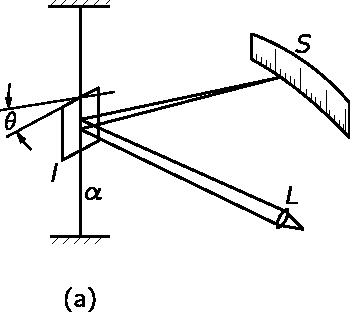
\includegraphics[width=0.7\linewidth]{fyz_fig483a.pdf}}  \\
     \subfloat[ ]{\label{fyz:fig483b}
       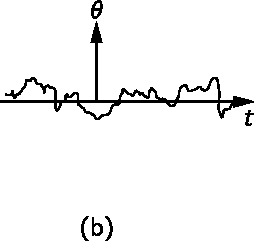
\includegraphics[width=0.6\linewidth]{fyz_fig483b.pdf}}  
    \end{tabular}
    \caption{
             (\cite[s.~601]{Feynman01}).}
    \label{fyz:fig483}
  \end{figure}

  \begin{figure}[hb!] %\ref{fyz:fig484}
    \centering
    \begin{tabular}{cc}
     \subfloat[ ]{\label{fyz:fig484a}
       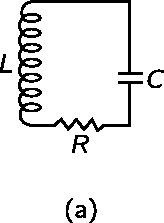
\includegraphics[width=0.4\linewidth]{fyz_fig484a.pdf}}  &
     \subfloat[ ]{\label{fyz:fig484b}
       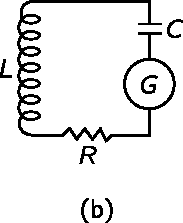
\includegraphics[width=0.4\linewidth]{fyz_fig484b.pdf}}
    \end{tabular}
    \caption{
             (\cite[s.~601]{Feynman01}).}
    \label{fyz:fig484}
  \end{figure}

    \begin{figure}[ht!] %\ref{fyz_fig485}
      \centering
      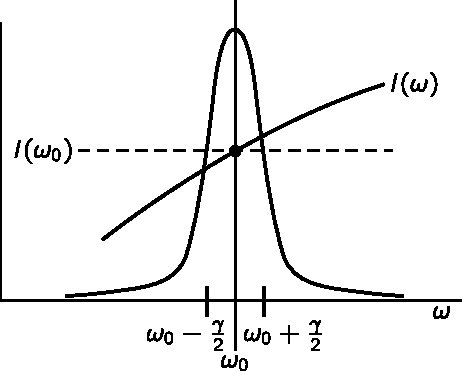
\includegraphics[width=0.7\linewidth]{fyz_fig485.pdf}
      \caption{ 
               (\cite[s.~707]{Feynman01})}
      \label{fyz_fig485}
    \end{figure}

    \begin{figure}[ht!] %\ref{fyz_fig486}
      \centering
      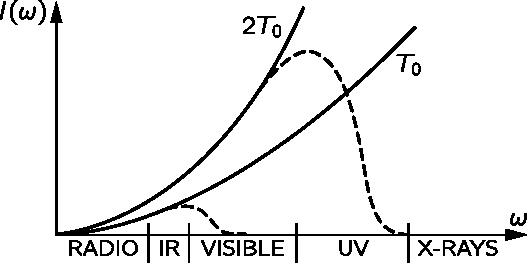
\includegraphics[width=0.7\linewidth]{fyz_fig486.pdf}
      \caption{ 
               (\cite[s.~707]{Feynman01})}
      \label{fyz_fig486}
    \end{figure}

    \begin{figure}[ht!] %\ref{fyz_fig487}
      \centering
      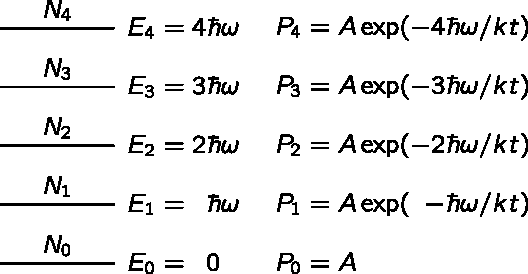
\includegraphics[width=0.7\linewidth]{fyz_fig487.pdf}
      \caption{ 
               (\cite[s.~707]{Feynman01})}
      \label{fyz_fig487}
    \end{figure}

    \begin{figure}[ht!] %\ref{fyz_fig488}
      \centering
      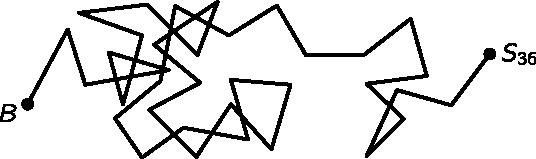
\includegraphics[width=0.7\linewidth]{fyz_fig488.pdf}
      \caption{ 
               (\cite[s.~707]{Feynman01})}
      \label{fyz_fig488}
    \end{figure}
    
    
} %tikzset
%---------------------------------------------------------------------------------------------------
\printbibliography[title={Seznam literatury}, heading=subbibliography]
\addcontentsline{toc}{section}{Seznam literatury}